\documentclass[12pt,a4paper]{article}
\pagenumbering{gobble} %remove page number
\usepackage[font=small,labelfont=bf]{caption} % Required for specifying captions to tables and figures
\usepackage{lmodern} %to fight font errors
\usepackage{array,booktabs,ragged2e}%centering tables 
\usepackage{polski}
\usepackage[utf8]{inputenc} 
\usepackage{blindtext}
\usepackage{longtable}
\usepackage[left=0.5cm,right=0.5cm,top=1cm,bottom=0.1cm]{geometry}
\usepackage{multirow}
\usepackage{verbatim}
\usepackage{multicol}
\usepackage{tabularray}
\usepackage{graphicx}
\usepackage{hyperref}
\hypersetup{colorlinks=true,linkcolor=blue,urlcolor=blue}

\usepackage{color}
\definecolor{techColor}{RGB}{120, 120, 120}

\newcolumntype{P}[1]{>{\centering\arraybackslash}p{#1}}

\begin{document}

\begin{tabular}  { >{\RaggedLeft}p{0cm} p{15.5cm}  p{2cm} }  
	& {\Large \textbf{KRZYSZTOF BOBNIS}} \hfill Wrocław & \textcolor{techColor}{residence} \\
	& GAME PROGRAMMER, GAME JAMMER \hfill  {\href{mailto:kbobnis@gmail.com}{kbobnis@gmail.com}} & \textcolor{techColor}{email} \\ 
	& \hfill {\href{https://www.linkedin.com/in/krzysztofbobnis}{linkedin.com/in/krzysztofbobnis}} & \textcolor{techColor}{linkedin} \\
	& \hfill {\href{http://bobnis.eu}{bobnis.eu}} & \textcolor{techColor}{portfolio} \\
\end{tabular}	 

\vspace{0.0cm}

\centering
\section*{Summary / Motivation}

	\begin{tabular}  { >{\RaggedLeft}p{0cm}  p{18cm}  p{0cm} }  

		 & Created a tool to produce adventure games that was used in multiple released projects already. Developed multiple successful mobile games. Created game prototypes on 20+ game jams. Believes that there is still a lot hidden potential in games, especially on big screen and comfortable controls. A true believer in honest feedback, following intuition, not being afraid of change. & \\
	\end{tabular}

\vspace*{1cm}

\begin{multicols}{2}

\section*{Experience }

	\begin{tabular}{ >{\RaggedLeft}p{0cm}   p{8.5cm}  } 
 
		&  \textbf{Tech Lead} / 2020 - Present \\
		&  \hspace{5mm}  {\href{https://dali.games/}{Dali Games}} - Created scriptless adventure game tool for unity. This common codebase was used to create two successful games: {\href{https://play.google.com/store/apps/details?id=games.dali.adventure.neighborhood.unholy}{Unholy Adventure (part 1, 2 and 3)}} 100,000+ installs and {\href{https://play.google.com/store/apps/details?id=games.dali.adventure.reborn}{Reborn Adventure}} 100,000+ installs.   \\

		& \\

		 & \textbf{Senior Game Programmer} / 2018 - 2020  \\
		& \hspace{5mm} {\href{https://cat-astrophe-games.com/}{Cat-astrophe Games}} - Created working prototype of run / walk / steps verifier as a game on a mobile phone. The client was happy with results and continued to invest in this prototype.  \\

		& \hspace{5mm} {\href{https://www.uken.com/}{Uken}}, Toronto, Canada  - Worked on a live video streaming game prototype with user interaction. Prior to that, developed Kings of Pool game {\href{https://play.google.com/store/apps/details?id=com.uken.pool}{Google play link}} with  500,000+ installs.  \\

		& \\
		&  \textbf{Game Programmer} / 2012 - 2017 \\ 
		& \hspace{5mm} {\href{https://tensquaregames.com/}{TSG}}, {\href{https://www.uken.com/}{Uken}} - Learned and applied frontend and backend technologies in as3, php, java, c\#, redis, mysql, git, svn to free to play web and mobile platforms. Game I was developing: Lets-Fish {\href{https://play.google.com/store/apps/details?id=air.com.tensquaregames.letsfish}{Google play link}} has 10,000,000+ installs.    \\	 

	\end{tabular}

\vfill

\section*{Education }
	\begin{tabular}{ >{\RaggedLeft}p{0cm}  p{8.5cm}   }

%& \\ 
		 & \textbf{Student} / 2006 - 2011: \\
		& \hspace{5mm}  \textbf{Graduated, Master of Science} in Information Technology. Wroclaw University of Technology, Major: Computer Science. Educational profiles: Artificial Intelligence, Advanced Computer Graphics, Computer Networks.   \\	 
	\end{tabular}


\section*{Achievements}
	\begin{tabular}  { >{\RaggedLeft}p{0cm}   p{8.5cm} }  
		& \textbf{Self publisher} / 2016 - Present: \\
		& \hspace{5mm} \textbf{Earned US\$10,000+} on my own game: {\href{https://play.google.com/store/apps/details?id=com.wyspianStudios.rpgModuleFull}{RPG Module - google play link}}   \\
		 & \\
%		\textbf{Co-organizer}  & Co-created and co-organized "Sensei" Game Jam, with 120 attendees in Wroclaw's University {\href{https://www.facebook.com/events/1110429105711126}{www.facebook.com/events/1110429105711126}}. & \\
		 & \textbf{Game Jammer} / 2013 - Present: \\
		& \hspace{5mm} \textbf{1st place} on TK Game Jam 2016. Finished on podium in several other game jams. Attended 20+ game jams in total. Created dozens of  games.  \\
	\end{tabular} 

\section*{Languages }
\begin{tabular}{ >{\RaggedLeft}p{0cm}  p{8.5cm}   }
	& \textbf{English}   \textbf{fluent}: relocated for 2 years to work as a game programmer in Toronto, Canada, passed ACERT: C1 english certificate  \\
	&  \textbf{Polish} \textbf{native}: born and live in Wroclaw \\	 
\end{tabular}

\vfill

\end{multicols}



\vfill

Some of my game jam entries (all are listed on my portfolio {\href{http://www.bobnis.eu}{http://www.bobnis.eu}}):
\begin{table}[htbp]
    \centering
    \begin{tblr}{
      colspec={X X X X X X }, row{1} = {c}, 
    }
		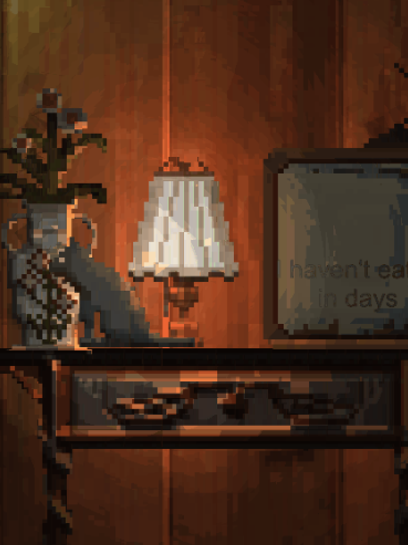
\includegraphics[height=3.0cm,width=1.75cm]{games/silence-of-the-cat.png}
		&  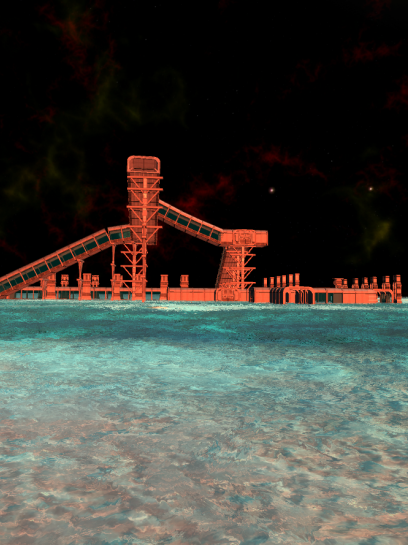
\includegraphics[height=3.0cm,width=1.75cm]{games/obrzed_przejscia.png}
		& 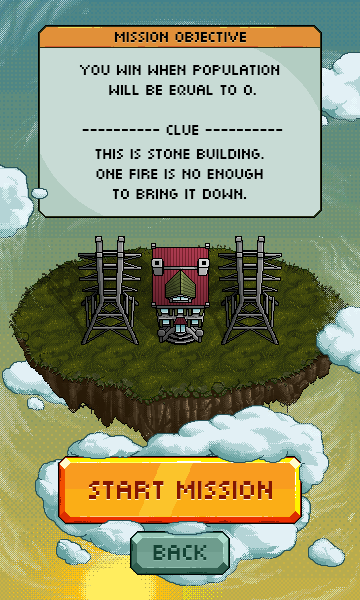
\includegraphics[height=3.0cm,width=1.75cm]{games/fog.png}
		& 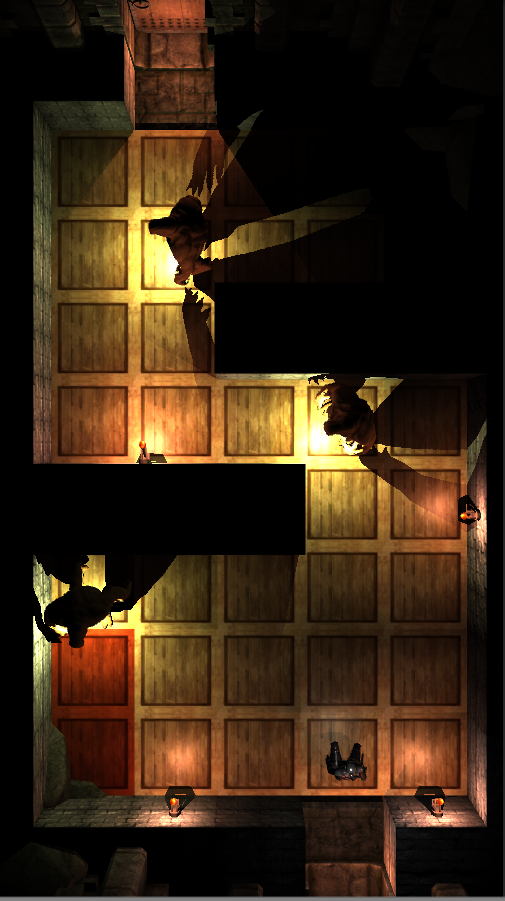
\includegraphics[height=3.0cm,width=1.75cm]{games/stealthRpg.png} 
		& 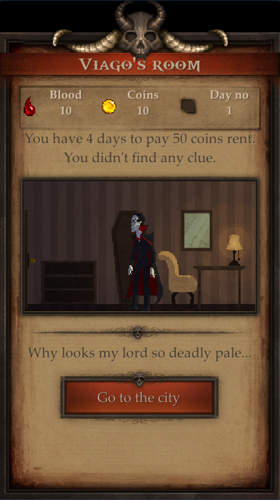
\includegraphics[height=3.0cm,width=1.75cm]{games/viago1.png} 
		&  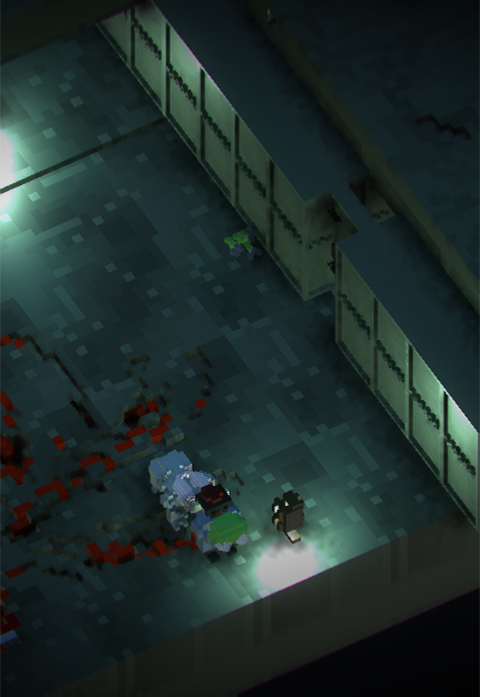
\includegraphics[height=3.0cm,width=1.75cm]{games/scp.png} \\

		  \centering Silence of the cat
		& \centering Obrzed przejscia
		& \centering Finger of God
		& \centering Stealth RPG
		& \centering Viago the Vampire
		& \centering SCP-35
    \end{tblr}
\end{table}


\end{document}
